\documentclass[12pt]{article}

\usepackage[english]{babel}
\usepackage[latin1]{inputenc}
\usepackage{times}
\usepackage{amsmath}
\usepackage{amssymb}
\usepackage{graphicx}
% 
%mise en forme document
%\setlength{\hoffset}{-18pt}\n";
\setlength{\oddsidemargin}{15pt}        % Marge gauche sur pages impaires\n";
\setlength{\evensidemargin}{15pt}       % Marge gauche sur pages paires\n";
\setlength{\marginparwidth}{54pt}       % Largeur de note dans la marge\n";
\setlength{\textwidth}{17cm}            % Largeur de la zone de texte (17cm)\n";
\setlength{\marginparsep}{7pt}          % Separation de la marge\n";
\setlength{\topmargin}{-20pt}           % Marge en haut\n";
\setlength{\headheight}{13pt}           % Haut de page\n";
\setlength{\headsep}{10pt}              % Entre le haut de page et le texte\n";
\setlength{\footskip}{2cm}              % Bas de page + separation\n";
\setlength{\textheight}{22cm} 
\usepackage[colorlinks=true, urlcolor=blue, linkcolor=blue]{hyperref}

\graphicspath{{pic/}}
%\setcounter{tocdepth}{2}
\usepackage{multirow}
\usepackage{longtable}
\usepackage{subfigure}
\usepackage[table]{xcolor}
\usepackage[absolute]{textpos} 

% Title Page
\title{\vspace{7cm}\textbf{ncPRO-seq}\\Annotation and Profiling of ncRNAs from smallRNA-seq\vspace{1.5cm} \normalsize ncPRO-seq version 1.3.0}
\date{\normalsize Last updated : \today}
\author{Chong-Jian Chen \& Nicolas Servant}
\def \ncpip{ncPRO-seq}

\clearpage
\begin{document}

\begin{titlepage}
\begin{center}
\begin{textblock*}{3cm}(8cm, 1cm)

\includegraphics[scale=0.8]{pic/ncPRO_logo.png}
\end{textblock*}
\end{center}
\end{titlepage}

\maketitle
\newpage

\tableofcontents
\clearpage
\section{Overview}
\subsection{Before starting}
\label{subsection:beforestarting}
Over recent years, deep sequencing technology has become a powerful approach for deeply investigating small non-coding RNA (ncRNA) populations, i.e. small RNA-seq. It is now established that an increasing number of novel small ncRNA families distinct from microRNAs are generated over kingdoms from different coding/non-coding regions via various biogenesis pathways and might involve a great spectrum of biological processes. For example, two other major classes of endogenous small RNAs, Piwi-interacting RNAs (piRNAs) and endogenous small interfering RNAs (endo-siRNAs), have been identified and widely investigated in mammals \cite{Ghildiyal2009}. Moreover, in other organisms like plants more classes of small ncRNA have been described indicating that a wide range of small ncRNAs exist \cite{Brodersen2006}.\\\\
However, most of the existing tools devoted to sRNA-seq analysis, are only based on miRNAs annotation and quantification, or can only be applied to one organism. Here we present a comprehensive and flexible ncRNA analysis pipeline, \textbf{\ncpip{}} (\textbf{\underline{N}}on-\textbf{\underline{C}}oding RNA \textbf{\underline{PRO}}filing in sRNA-\textbf{\underline{seq}}) (http://ncproseq.sourceforge.net), which is able to interrogate and perform detailed analysis on small RNAs derived from annotated non-coding regions in miRBase \cite{Kozomara2011}, Rfam \cite{Gardner2011} and repeatMasker \cite{Smit2008}, and regions defined by users. The \ncpip{} pipeline also has a module to identify regions significantly enriched with short reads that can not be classified as known ncRNA families. The ncPRO-seq pipeline supports input read sequences in fastq, fasta and color space format, as well as alignment results in BAM format, meaning that small RNA raw data from the 3 current major platforms (Roche-454, Illumina-Solexa and Life technologies-SOLiD) could be analyzed with this pipeline. Finally, the ncPRO-seq pipeline can be used to analyze data based on genome from metazoan to plants.
\subsection{About us}
\ncpip{} is developped in the context of a collaborative project involving the following partners :
\begin{itemize}
\item Institut Curie - Platforme Bioinformatique (France, Paris)
\item G�n�tique et biologie du d�veloppement (France, Paris) - Institut Curie - UMR 3215 CNRS - U934 Inserm 
\item Arabidopsis Epigenetics and Epigenomics group (France, Paris) - CNRS UMR8197 - INSERM U1024 - Institut de Biologie de l'Ecole Normale Sup�rieure 
\item Institut de Biologie Mol�culaire des Plantes du CNRS - UPR2357 (France, Strasbourg)  
\item Department of Biology - Swiss Federal Institute of Technology Zurich (Suisse, Zurich)  
\end{itemize}

\noindent If you use the ncPRO-seq tool for your analysis, please cite the following paper :\\
Chen C., Servant N., Toedling J., Sarazin A., Marchais A., Duvernois-Berthet E., Cognat V., Colot V., Voinnet V., Heard E., Ciaudo C. and Barillot E. \textit{ncPRO-seq: a tool for annotation and profiling analysis of ncRNAs from small RNA-seq.} submitted. 


\section{Requirements and Installation}
\subsection{Hardware}
Computer with at least 4GB of primary memory is recommended. Although the \ncpip{} pipeline is fast ($\sim$1h30 for 10 million reads) in a simple desktop computer or laptop, launching the pipeline in a computer cluster would achieve much better performance by turning on the multithreading option.
\subsection{Operating system}
In the current version, the \ncpip{} pipeline can only be installed in a Linux/UNIX-like operating system (Linux/UNIX or Mac OS X).
\subsection{Required softwares}
The \ncpip{} pipeline requires the following additional softwares. Please refer to section \ref{subsection:additional} for more details :

\begin{itemize}
 \item The \href{http://bowtie-bio.sourceforge.net/manual.shtml}{ Bowtie Aligner} ($<$v2.0) \cite{Langmead2009} to align the reads from smallRNA-seq data.

 \item The \href{http://www.r-project.org/}{ R} ($>$v2.12.0) \cite{Rcitation}.

 \item The R and \href{http://www.bioconductor.org/}{ BioConductor} \cite{Robert2004} packages:  \href{http://www.bioconductor.org/packages/2.2/bioc/html/seqLogo.html}{ seqLogo} \cite{OliverseqLogo}, \href{http://www.bioconductor.org/packages/2.6/bioc/html/girafe.html}{ girafe} \cite{Joern2010} and  \href{http://cran.r-project.org/web/packages/RColorBrewer/index.html}{ RColorBrewer} \cite{Erich2011}.

 \item The \href{http://code.google.com/p/bedtools/}{ BEDTools suite}  ($>=$v2.15.0) \cite{Quinlan2010}, and the \href{
http://xfer.curie.fr/get/nil/2Rpz9IfJKcZ/BEDTools_MapCount_ColorTag.tar.gz }{ bamMapCount} program  to address common genomic tasks such as finding feature overlaps and grouping same features.

 \item The \href{http://samtools.sourceforge.net/}{ SAMTools suite} \cite{Li2009} to handle SAM and BAM format.

 \item The \href{http://www.imagemagick.org/script/index.php}{ Convert/ImageMagick} utilies to format files and images.

 \item In order to use the end-user interface, a local server with php such as apache is needed.

 \item For Mac OS X user, make sure that you have \href{http://developer.apple.com/xcode/}{ Xcode} installed in your system.
\end{itemize}

\noindent
\subsection{Installation of \ncpip{}}
You can download the source of \ncpip{} and annotation files of different species from our project page in sourceforge (http://sourceforge.net/projects/ncproseq/files/).\\\\
To build the \ncpip{} pipeline, extract the source and species annotation file you choose, move the whole folder of species annotation files to annotation/ in the sources folder. \\Edit the \verb+config-system.txt+ file in the sources folder and change the paths of the required softwares.
\label{subsection:configsys}

\begin{center}
\rowcolors{1}{white}{gray!20}
\begin{longtable}{|p{5cm}|p{5cm}|p{6cm}|}
\hline \rowcolor{gray} 
\textbf{Options}&\textbf{Description}&\textbf{Example}\tabularnewline 
\textbf{INSTALL\_WWW} & 0/1. If 1, the web interface of \ncpip{} is installed in \textbf{WWW\_DIR} and \textbf{CGI\_DIR}&1\\
\textbf{APPLI\_DIR} & Absolute path of installation folder&/home/ncPROseq/\\
\textbf{WWW\_DIR} & HTML installation folder. Have to be under the web working directory&/var/www/ncPROseq/\\
\textbf{CGI\_DIR} & CGI installation folder. Have to be under the CGI working directory&/usr/lib/cgi-bin/ncPROseq/\\
\textbf{WWW\_RES} & Results path for local web version & /home/ncPROseq/www\_results\\
\textbf{PBS\_MODE} & 0/1. If 1, the job are send to the PBS job scheduler using the \textit{qsub} command & 0\\
\textbf{PBS\_OPT} & Options to give to \textit{qsub} at job submission & -m ae -M bioinfo.ncproseq@curie.fr -j oe -l nodes=1:ppn=6,mem=20gb\\
\textbf{PBS\_PATH} & Absolute path to PBS (qsub) command & /usr/bin\\ \hline

\textbf{R\_PATH} & Absolute path to R binary folder&/usr/local/R/R/bin/\\
\textbf{AWK\_PATH} & Absolute path to awk executable folder & /usr/bin/\\
\textbf{BOWTIE\_PATH} & Absolute path to bowtie executable folder & /usr/local/bowtie-0.12.7/\\
\textbf{BOWTIE\_INDEXES\_PATH} & Installation folder of Bowtie indexes & /home/Apps/Bowtie\_indexes/\\
\textbf{BEDTOOLS\_PATH} & Installation folder of BedTools binaries & /home/Apps/BEDTools-Version-2.15.0/bin/\\
\textbf{SAMTOOLS\_PATH}  & Installation folder of samtools binary & /home/nservant/Apps/samtools/ \\
\textbf{CONVERT\_PATH}  & Utilities used to create thumbnail for html report&/usr/bin/ \\
\textbf{BAM\_MAPCT\_PATH}  & Installation folder of the bamMapCount program. Distributed with the BEDTools-version10.0& /home/Apps/BEDTools-Version-2.10.0/bin/\\
\textbf{PERL\_PATH} & Perl installation folder& /usr/local/bin \\
\textbf{MAILX\_PATH} & Optional - mailx excutable path to send email at the end of the analysis&/usr/bin/\\
\hline
\caption{Set Paths in the config-system.txt file before installation.}
\label{tab:configsysoptions}
\end{longtable}
\end{center}

Once the \verb+config-system.txt+ is ready, go to the sources directory, and simply use the following command:\\
\begin{verbatim}
> make CONFIG_SYS=config-system.txt install
\end{verbatim}

This command will install the sources in the folder specified in the \verb+config-system.txt+ file. Note that if some of the paths from the config-system.txt are not correct (or unknown), the installation program will try to find them on the system.\\
In most of the cases, the installation of \ncpip{} required \textbf{administrator rigths}, especially for the installation under the web directories.

\section{How to use it ?}

\subsection{Configuration file}
\ncpip{} is a flexible pipeline which allows users to specify different options at each analysis stage, from raw reads processing to ways to generate results. In the web interface version, all options can be easily chosen through the web (see \ref{subsection:webinterface}). In command line version (see \ref{subsection:commandline}), users can manually edit the \verb+config-ncrna.txt+ file to define options according to the descriptions of options below (Table ~\ref{tab:configureoptions}) and also inside the file. In the \verb+config-ncrna.txt+ file, you may find more options than that in the web page, especially for the Bowtie mapping step, but we do not suggest you to make any changes in these extra options unless you are an expert.\\\\

\label{subsection:configure}

\begin{center}
\rowcolors{1}{white}{gray!20}
\begin{longtable}{|p{8cm}|p{8cm}|}
\hline \rowcolor{gray} 
\textbf{Options}&\textbf{Description}\tabularnewline 
\textbf{LOGFILE} & File that lists actions that have occurred during the analysis\\
\textbf{N\_CPU}& Number of CPU used by Bowtie to do mapping\\
\textbf{FASTQ\_FORMAT} & The quality score format of the fastq reads. Three formats are supported: \textbf{phred33} (Sanger, Solexa version 1.8 or later), \textbf{solexa} (Solexa prior to version 1.3), \textbf{solexa1.3} (Solexa version 1.3 to 1.7)\\
\textbf{BOWTIE\_GENOME\_REFERENCE} & Basename of the Bowtie index genome reference file (base space). See the \href{http://bowtie-bio.sourceforge.net/manual.shtml}{ Bowtie manual} for additional informations\\
\textbf{BOWTIE\_GENOME\_REFERENCE\_CS} & Basename of the Bowtie index genome reference file (color space). See the \href{http://bowtie-bio.sourceforge.net/manual.shtml}{ Bowtie manual} for additional informations\\
\textbf{BOWTIE\_GENOME\_OPTIONS\_FQ} & Options for Bowtie to map base space reads in fastq format (Solexa)\\
\textbf{BOWTIE\_GENOME\_OPTIONS\_FA} & Options for Bowtie to map base space reads in fasta format (454)\\
\textbf{BOWTIE\_GENOME\_OPTIONS\_CS} & Options for Bowtie to map color space reads (SOLiD)\\
\textbf{GROUP\_READ} &  Group reads based on their sequence for raw reads before mapping or read alignments in bam file depending on the input format. \textbf{1}: Yes; \textbf{0}: No; \textbf{2}: for the online version where the input files have already been grouped using our provided scripts\\ 
\textbf{ORGANISM} & Name of the reference organism. Must be the same as the organism available in the annotation folder (i.e. mm9, hg19, ...)\\
\textbf{MATURE\_MIRNA} & Annotation against miRNAs from miRBase. Both miRNA with and without an extended item are acceptable (see \ref{subsubsection:extension})\\
\textbf{PRECURSOR\_MIRNA} & Annotation against pre-miRNAs from miRBase. Both miRNA with and without an extended item are acceptable (see \ref{subsubsection:extension})\\
\textbf{NCRNA\_RFAM} & List of the RFAM ncRNA(s) to focus on (comma separator) - no extension parameter\\
\textbf{NCRNA\_RFAM\_EX} & List of the RFAM ncRNA(s) to focus on (comma separator) - extension parameter (see \ref{subsubsection:extension})\\
\textbf{NCRNA\_RMSK} & List of the repetitive elements to focus on (comma separator) - no extension parameter \\
\textbf{NCRNA\_RMSK\_EX} &  List of the repetitive elements to focus on (comma separator) -  extension parameter (see \ref{subsubsection:extension})\\
\textbf{TRNA\_UCSC} & Mapping against tRNA sequences. Both tRNA with and without an extended item are acceptable (see \ref{subsubsection:extension})\\
\textbf{OTHER\_NCRNA\_GFF} & List of custom gff files to intersect with the mapped reads\\
\textbf{LOGO\_DIRECTION} &  Align the sequence on the 5' or 3' end \textbf{[5/3]}\\
\textbf{IC\_SCALE} & Use the information content scale for Logo outputs. \textbf{1}: Yes; \textbf{0}: No\\
\textbf{GENOME\_TRACK\_OPTIONS} & Options to select reads mapped in the genome to generate track file. Four options should be provided to filter reads, and separated by comma. \textbf{min\_len=N} : the minimum length (N) of read; \textbf{max\_len=N}: the maximum length (N) of read; \textbf{min\_copy=N} : the minimum number (N) of matches in the genome; \textbf{max\_copy=N}: the maximum number (N) of matches in the genome. To have more than one type of track, different sets of options should be separated by pipe ($|$)\\
\textbf{SIG\_READ\_OPTIONS} & Options to select mapped reads for enrichment analysis (see \ref{subsection:enrichmentanalysis}). Please refer to the format of \textbf{GENOME\_TRACK\_OPTIONS}\\
\textbf{SIG\_WIN\_SIZE} & The window size used to scan the genome (e.g. 10000) (see \ref{subsection:enrichmentanalysis})\\
\textbf{SIG\_STEP\_SIZE} & The step size (e.g. 50000) (see \ref{subsection:enrichmentanalysis})\\
\textbf{EXCLUDE\_ANN\_GFF} & List of annotation files (gff3). Only reads which are not mapped in these annotated regions are kept for enrichment analysis (see \ref{subsection:enrichmentanalysis})\\
\textbf{FIT\_MODEL} & The model used to fit window-based read distribution. Three models can be chosen: \textbf{NB.ML}, \textbf{NB.012}, and \textbf{Poisson} (see \ref{subsection:enrichmentanalysis})\\
\textbf{PVAL\_CUTOFF} & The cut-off used to get regions significantly enriched with reads\\
\hline
\caption{Options from the configuration file}
\label{tab:configureoptions}
\end{longtable}
\end{center}

\subsection{Web interface version}
\label{subsection:webinterface}
The \ncpip{} pipeline provides a local web interface to run the analysis. Most of the options describe in the section~\ref{subsection:configure} can be defined using the interface. To open the \ncpip{} interface, just enter the web url (as defined in \verb+WWW_DIR+ in the configuration system file), followed by the \verb+load.php+ file. For instance, open http://localhost/ncPROseq/load.php in your favourite navigator.\\
This web implementation uses a Perl CGI scripting program, and required perl to be installed in /usr/bin/perl. This path is the default path under Unix system. If not available, please ask your administrator to create a link to your own perl environment.

\subsubsection{Input data files}
The local input files can be selected as shown in Figure~\ref{fig:web1}. As previously described, the .fastq, .csfasta, and .fasta raw sequencing data can be selected, as well as .bam files for reads already aligned on the genome. These different file types can be mixed in a single analysis.\\
If a folder is selected, all the files within the folder will be analysed.
In order to avoid security issues (i.e. browsing the entire file server), \textbf{the user has to enter the full path of its data}.
As any standard web application, \ncpip{} is run by the http user. Accordingly, \textbf{it is your responsabilities to check if the http user can read your data}.


\begin{figure}[!h]
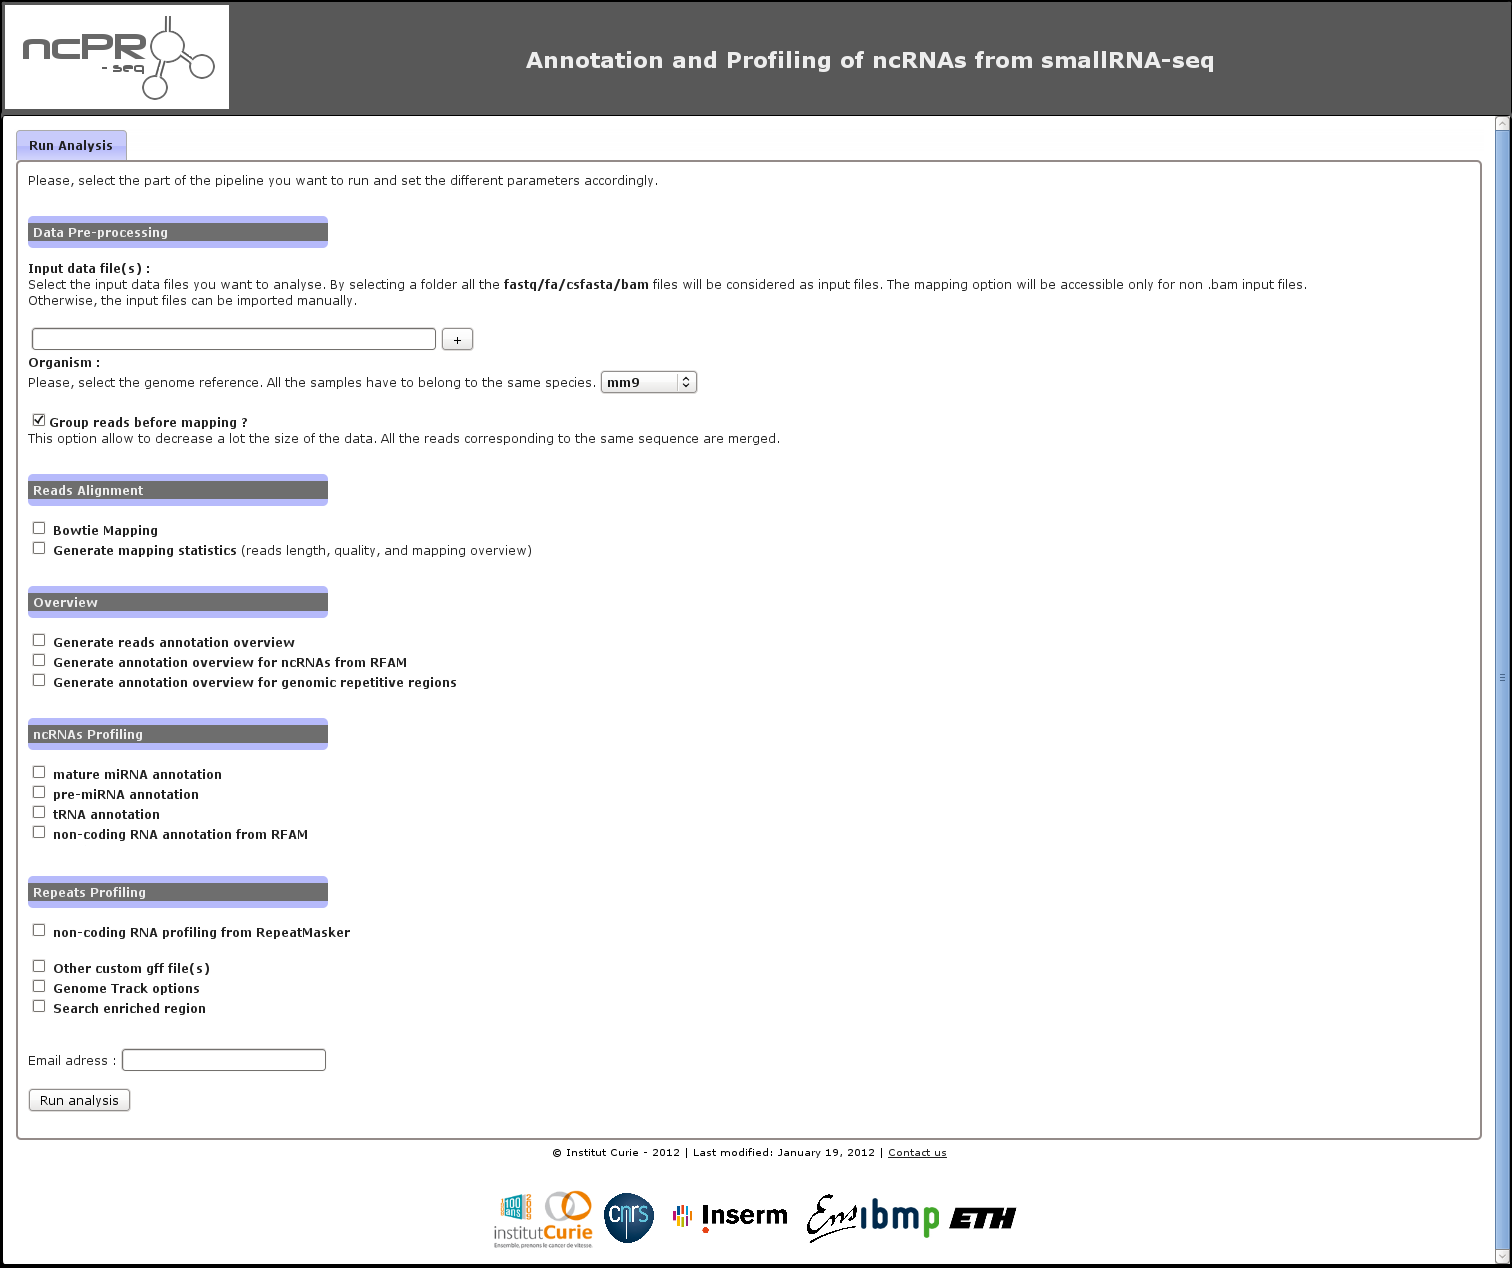
\includegraphics[width=\textwidth]{web_1.png}
\caption{\ncpip{} web interface: load input files}
\label{fig:web1}
\end{figure} 
\subsubsection{Alignment on a reference genome}
The Figure~\ref{fig:web2} presents the different parameters to set for the short reads mapping using the Bowtie alignment tool.\\
First, the user has to select if the reads has to be grouped before mapping (see section~\ref{subsubsection:readpreprocess}). We highly recommended to use this option, as it reduces a lot the size of the input reads (and output files), and have only very few impact (if any) on the results. All the reads corresponding to the same sequence are merged, and the related quality values are averaged.\\
\begin{figure}[!h]
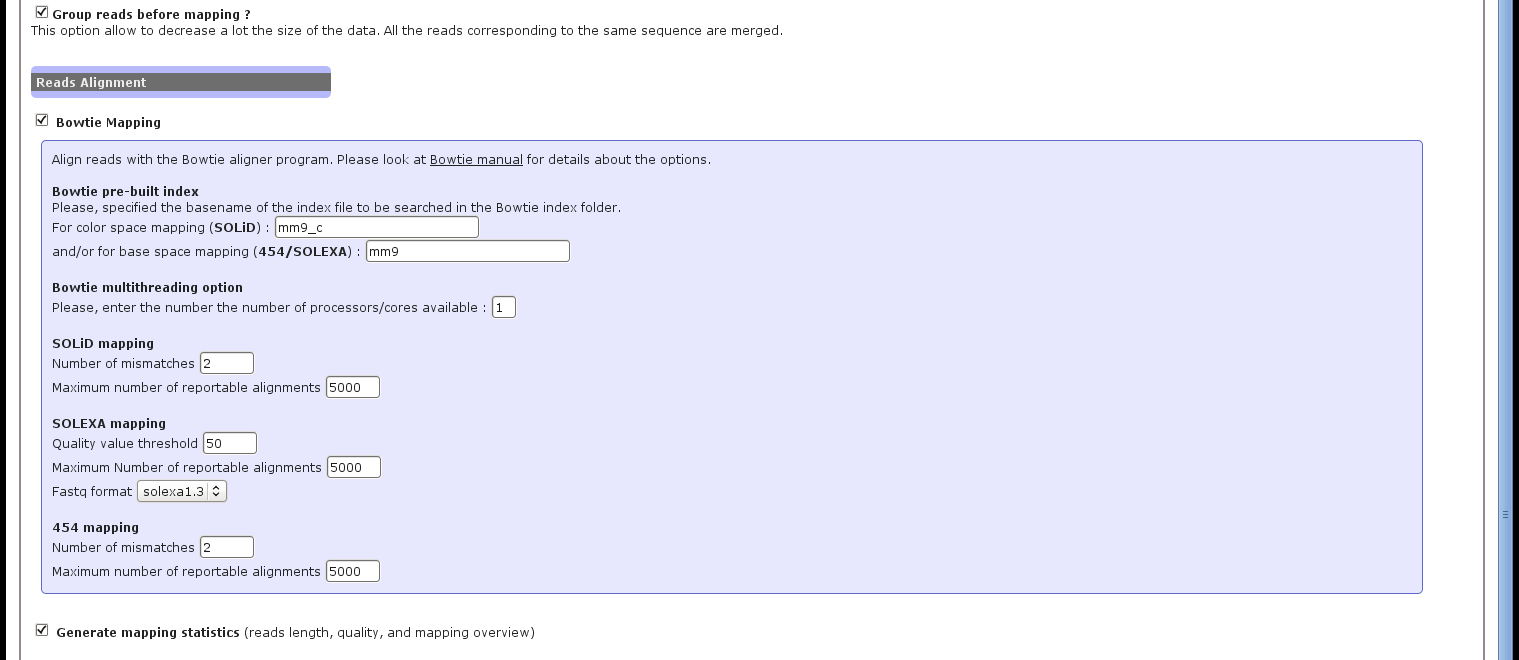
\includegraphics[width=\textwidth]{web_2.png}
\caption{\ncpip{} web interface: set alignment parameters}
\label{fig:web2}
\end{figure} 
The following Bowtie options can then be available. For details explanation, please see the \href{http://bowtie-bio.sourceforge.net/manual.shtml}{ Bowtie manual page}.

\begin{itemize}
\item \textbf{Bowtie pre-built index.} The name of the index file to be searched in the Bowtie index folder (as specified in the system configuration file during installation). 
\item \textbf{Mapping options.} Using the interface, all input file are aligned with the options '-a --best --strata -y' to always select the best hits. Then, the number of mismatches (up to 3), the maximum number of reportable alignments or the fastq format have to be choose according to the input data type, and the goal of the analysis. 
\item \textbf{Bowtie multithreading option.} Number of CPUs used by Bowtie to perform the alignment.
\end{itemize}
Finally, the user can also ask for a quality mapping report. In this case, the following outputs are generated :
\begin{itemize}
\item Reads length distribution.
\item Sequence length distribution (only the distinct reads are used).
\item Number of reads aligned on the genome reference.
\end{itemize}

\subsubsection{Annotation Overview}
The overview section aims in annotating the reads and classifying them into large families (see the section~\ref{subsubsection:overview}).\\
The reads annotation family is the most general view, and annotates the reads based on the following annotations : coding genes, ncRNAs from Rfam, smallRNAs from repeated regions, rRNA, and precursor miRNA from miRBase. Please, note that \ncpip{} uses the miRBase annotation for miRNAs, and that accordingly, the miRNAs from Rfam are not used.\\
Then, an overview of the non-coding RNAs annotation and of the repetitive genomic regions are provided.
\begin{figure}[!h]
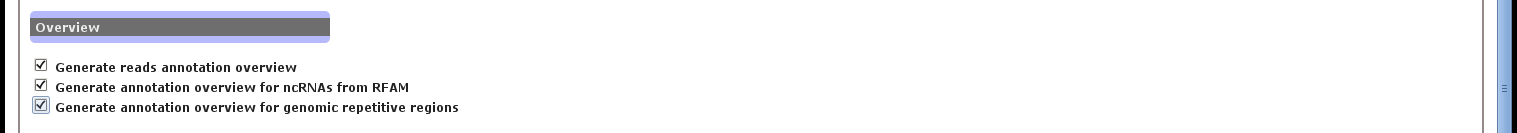
\includegraphics[width=\textwidth]{web_3.png}
\caption{\ncpip{} web interface: reads annotation}
\label{fig:web3}
\end{figure} 

\subsubsection{Profiling of non-coding RNAs}
Then, the profiling of the non-coding RNAs (section ~\ref{subsubsection:readprofile}) can be performed by selecting the RNAs classes to focus on and the associated extension parameters as presented in section~\ref{subsubsection:extension} (Figure~\ref{fig:web3}).
Regarding the ncRNAs from the RFAM database, several targets can be specified. The profiling analysis will be separately done for each input keyword.\\
\begin{figure}[!h]
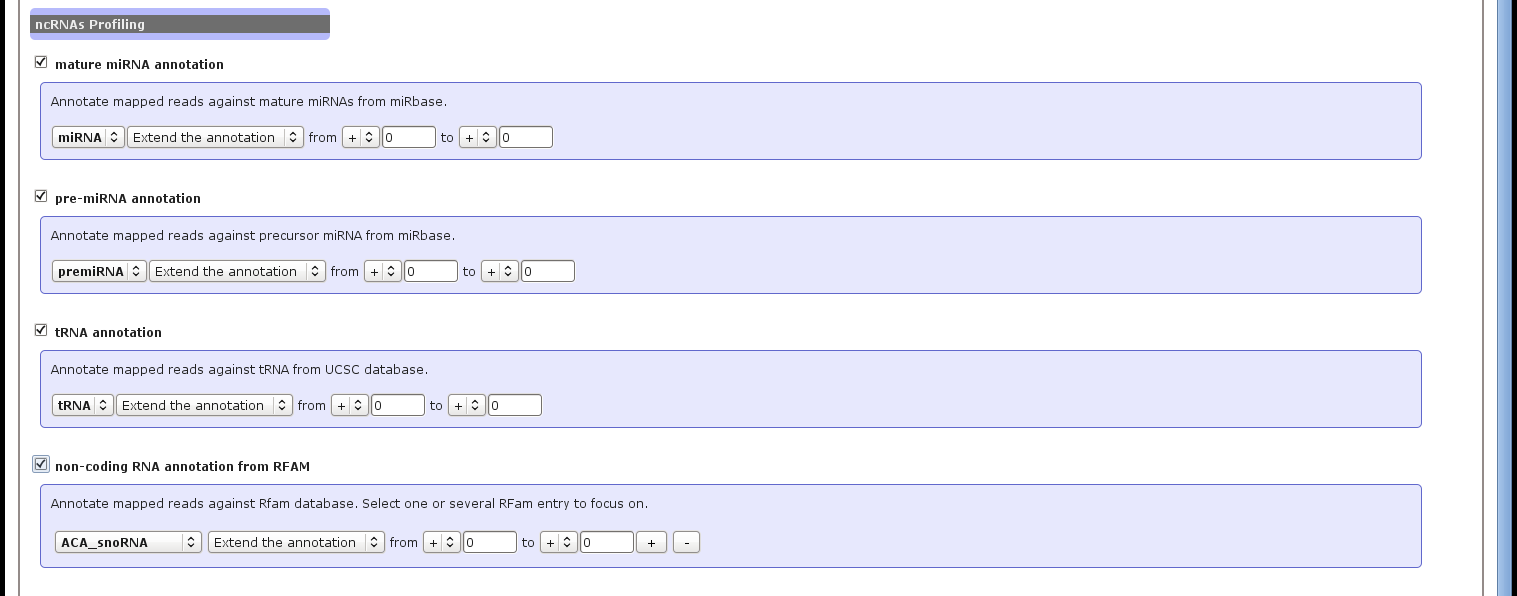
\includegraphics[width=\textwidth]{web_4.png}
\caption{\ncpip{} web interface: annotation of ncRNAs}
\label{fig:web3}
\end{figure} 
\subsubsection{Profiling of repetetive regions}
The same profiling options are available for the annotation of the repetitive genomic regions (Figure~\ref{fig:web5}). Here, \ncpip{} offers the possibility to select only full length repeated elements. The full length elements are detected using the position of each element on the consensus sequence (data from UCSC). Only the elements matching the exact length of the consensus are considered as full length. 
\begin{figure}[!h]
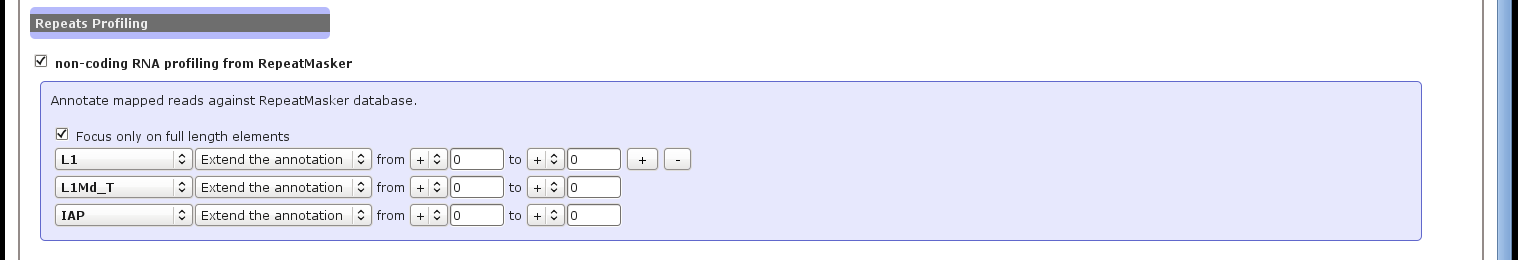
\includegraphics[width=\textwidth]{web_5.png}
\caption{\ncpip{} web interface: annotation of repetitive regions}
\label{fig:web5}
\end{figure}
\subsubsection{User Custom gff files}
For each annotation family including different repeat/Rfam families and other custom annotations, \ncpip{} creates a table file showing read coverages of each single family member in all sequencing libraries. If some annotations are not available, or if the user want to search for reads annotated in other genomcis regions, the profiling can also be done on custom gff files. As for the input files, the full path of the gff files has to be set. Several custom gff files can be specified.

\subsubsection{Genome tracks visualisation}
For each sequencing library,  for each annotation family, \ncpip{} generates two compressed track files in \href{http://genome.ucsc.edu/goldenPath/help/bedgraph.html}{bedgraph} and \href{http://genome.ucsc.edu/FAQ/FAQformat.html#format1format}{bed} formats to describe read mapping in sense and antisense direction of annotation items respectively. These track files can be then, easily upload in a visualisation tool as the UCSC Genome Browser \cite{Dreszer2012}.\\
Moreover, the interface allows users to select different subsets of reads mapped in the genome to generate BedGraph formatted track files.
The minimum and maximum size of the reads, as well as the minimum and maximum number of locations can be used to filter the aligned reads (Figure~\ref{fig:web6}).
\begin{figure}[!h]
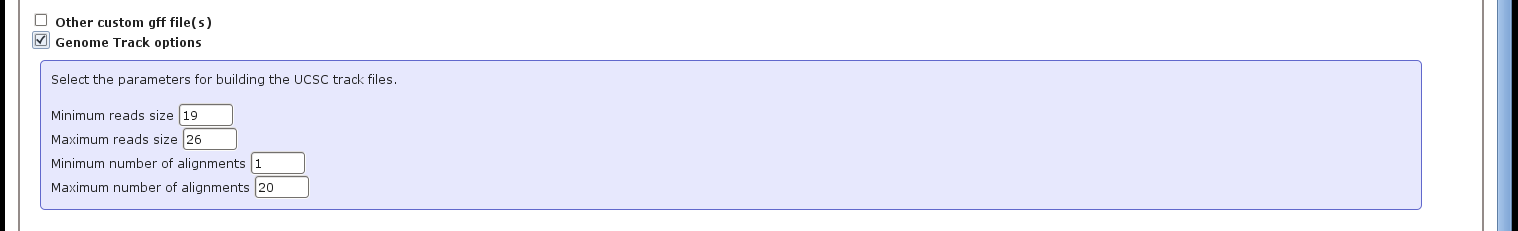
\includegraphics[width=\textwidth]{web_6.png}
\caption{\ncpip{} web interface : genome tracks options}
\label{fig:web6}
\end{figure}
\subsubsection{Search enriched regions}
The enrichment analysis can be launch from the interface, by specifying the different options as explained in the section~\ref{subsection:enrichmentanalysis}.
As for the Genome tracks options, the user can choose to focus on a subset of reads. The minimum and maximum size of the reads, as well as the minimum and maximum number of locations can be used to select these reads. Then only the reads not annotated on the selected items (coding genes, miRNAs, ncRNAs) will be used for the analysis (Figure~\ref{fig:web7}).
\begin{figure}[!h]
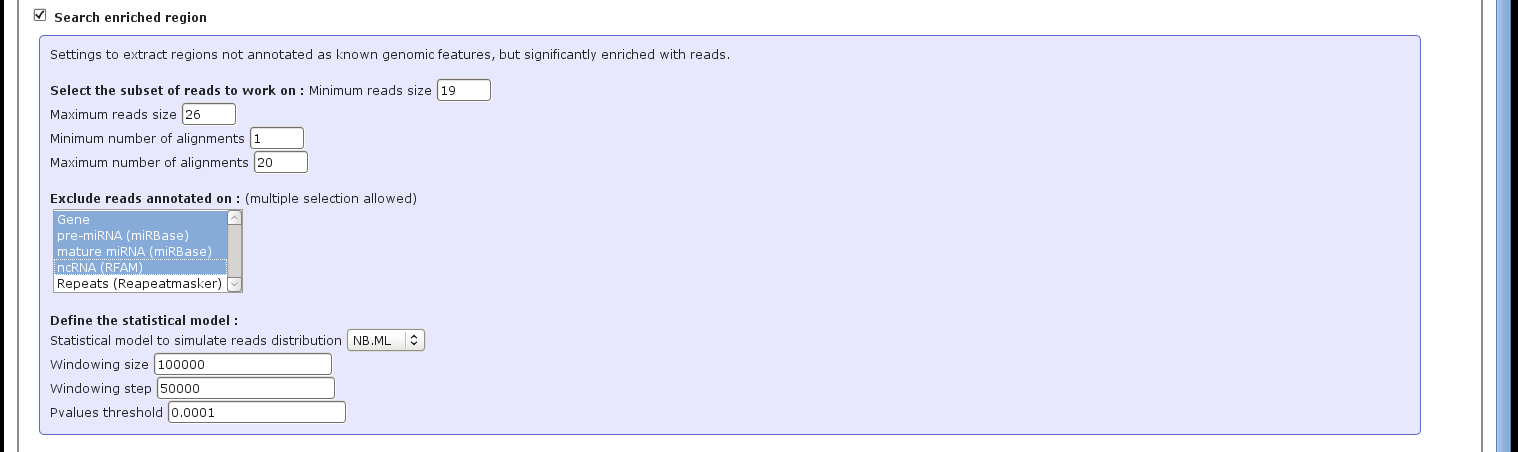
\includegraphics[width=\textwidth]{web_7.png}
\caption{\ncpip{} web interface : search enriched regions}
\label{fig:web7}
\end{figure}
\subsubsection{Run the analysis}
Finally, after setting the different parameters, the \ncpip{} pipeline can be executed. A random url will be generated (Figure~\ref{fig:web8}) to visualize the output report (see section~\ref{section:report}). If specified, an email will be send to the user at the end of the analysis.\\
Please, note that in the current version the report will be updated only \textbf{at the end} of the analysis.
\begin{figure}[!h]
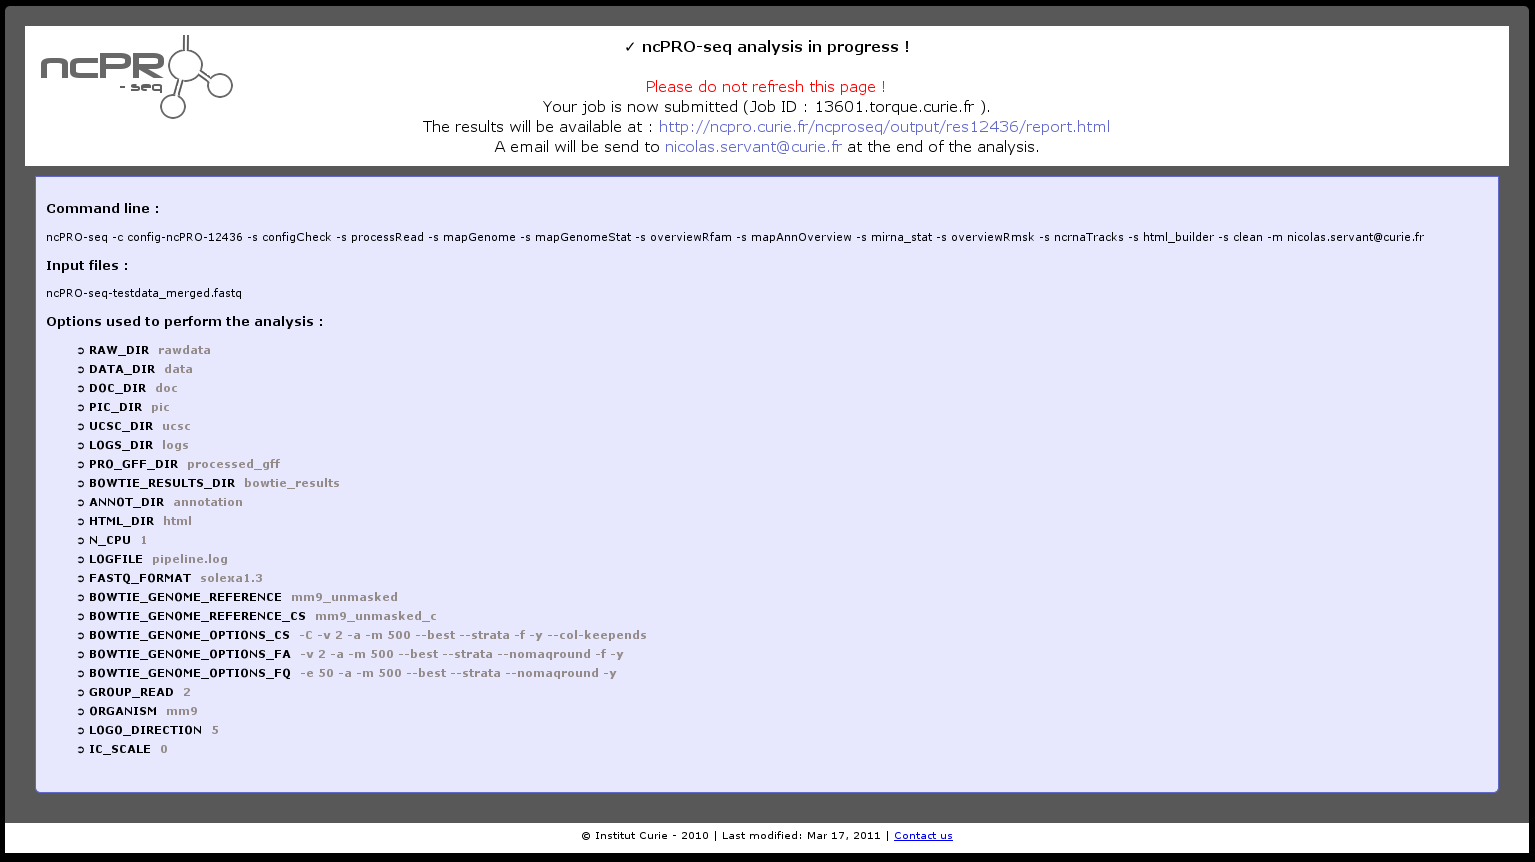
\includegraphics[width=\textwidth]{web_8.png}
\caption{\ncpip{} web interface: run the analysis}
\label{fig:web8}
\end{figure}
\newpage
\subsection{Command-line version}
\label{subsection:commandline}
The \ncpip{} pipeline will generate a lot of output files. Thus before starting, it is highly recommended to deploy the \ncpip{} output architecture.\\
However, this step is \textbf{optional}. If you don't want to use this output architecture, please change the output paths in the configuration files.
To deploy the output architecture, use the following command:
\begin{verbatim}
$ MY_INSTALLATION_DIR/bin/ncPRO-deploy -o MY_OUTPUT_DIR
\end{verbatim}

The input (fastq, bam, csfasta or fasta) files must be filed in the rawdata folder.
Finally, after setting the different parameters in the configuration file, run the ncPRO-seq pipeline as follow : 
\begin{verbatim}
$ cd MY_OUTPUT_DIR
$ MY_INSTALLATION_DIR/bin/ncPRO-seq -c config-ncrna.txt
\end{verbatim}

The \ncpip{} pipeline is modular and sequential. The user can specify the analysis steps to run.
For instance, the following command line will just perform the quality control, the reads grouping, and the alignment on the reference genome.
\begin{verbatim}
$ MY_INSTALLATION_DIR/bin/ncPRO-seq -c config-ncrna.txt -s processRead 
-s mapGenome -s mapGenomeStat 
\end{verbatim}
The following analysis steps are available:
\begin{center}
\rowcolors{1}{white}{gray!20}
\begin{longtable}{|p{8cm}|p{8cm}|}
\hline \rowcolor{gray} 
\textbf{\ncpip{} analysis step (-s option)} &	\textbf{Description}\tabularnewline 
processRead &	calculate read length distribution, median quality score for each postion, and group reads\\
processBam &	processed and group reads from bam files\\
mapGenome &	run Bowtie for genome mapping\\
mapGenomeStat&	compute number of mapped reads and unmapped reads in the genome\\
mapAnnOverview & compute overview of reads annotation\\
overviewRmsk &	compute read coverage for each repeats family\\
overviewRfam &	compute read coverage for each ncRNA family\\
generateNcgff &	create gff file for special ncrna family\\
ncrnaProcess&	ncRNA family analyses, including read coverage, read length distribution, read coverage in subfamilies, and sequence logo\\
genomeTracks & genreate genome coverage ucsc track\\
ncrnaTracks & genreate ucsc tracks for ncrna visualization\\
sigRegion &	detect significantly enriched regions\\
html\_builder &	build the html report file\\
\hline
\caption{Description of \ncpip{} '-s' options}
\label{tab:configureoptions}
\end{longtable}
\end{center}

\section{How to browse the results ?}
\label{section:report}

Users just need to open "report.html" automatically created by \ncpip{} in a web browser to easily view figures and tables which are originally stored in \verb+pic+ (for pictures) and \verb+doc+ (for table files) folder respectively, and to access track files in UCSC folder (Figure ~\ref{fig:report}). The report file is composed of 7 types of tab. Briefly, each tab presents the pictures (or tables) generated by the pipeline. Each picture, and table can be visualized in high resolution, and/or download for further analysis. 
\begin{description}
 \item[Home.] The main page of the report list all samples and options used to perform the analysis, and the version of pipeline, used softwares and annotation files.
 \item[Quality Control.] All the quality controls performed on the raw input data are presented in this tab. The mean quality score, base, GC, and the insert length distribution are available.
 \item[Data Mapping.] As for the quality control, all the pictures regarding the alignment of reads on the reference genome are presented here. The reads length distribution, and the mapping proportion are available. These first controls give a good idea of the overall quality of the input libraries.
 \item[ncRNAs Overview.] The annotation overview of the different ncRNAs family is separated in pre-miRNAs, rRNA, repeat, rfam, protein coding gene and unknown. For the RFAM/repeats annotation, the \ncpip{} pipeline count the number of abundant reads in each family and provides the relative proportion.
 \item[ncRNAs Profiling.] Then, for each ncRNAs specified in the configuration file (see section~\ref{subsubsection:extension}), and each samples, \ncpip{} generate the coverage profile and the logo sequences. As for most of the analysis, both results at the reads or the sequence level are available. Regarding the logo sequences, both view (all sequences, or major sequence) are available (see section~\ref{subsubsection:logo}).
 \item[Table view.] All the table files generated by the \ncpip{} pipeline can be browsed, visualized, and downloaded. The files are organized from general overview, to ncRNAs profiling information.
 \item[Genome Tracks.] The bedgraph or bed files generated by the pipeline can be downloaded and loaded in a standard visualisation tool, such as the \href{http://genome.ucsc.edu/index.html}{ UCSC browser} \cite{Dreszer2012}
 \item[Logs.] The log file of the \ncpip{} process is printed here. Check this file in case of error.
 \item[Help.] This manual is available trough the report interface.
 \end{description}

\begin{figure}[!h]
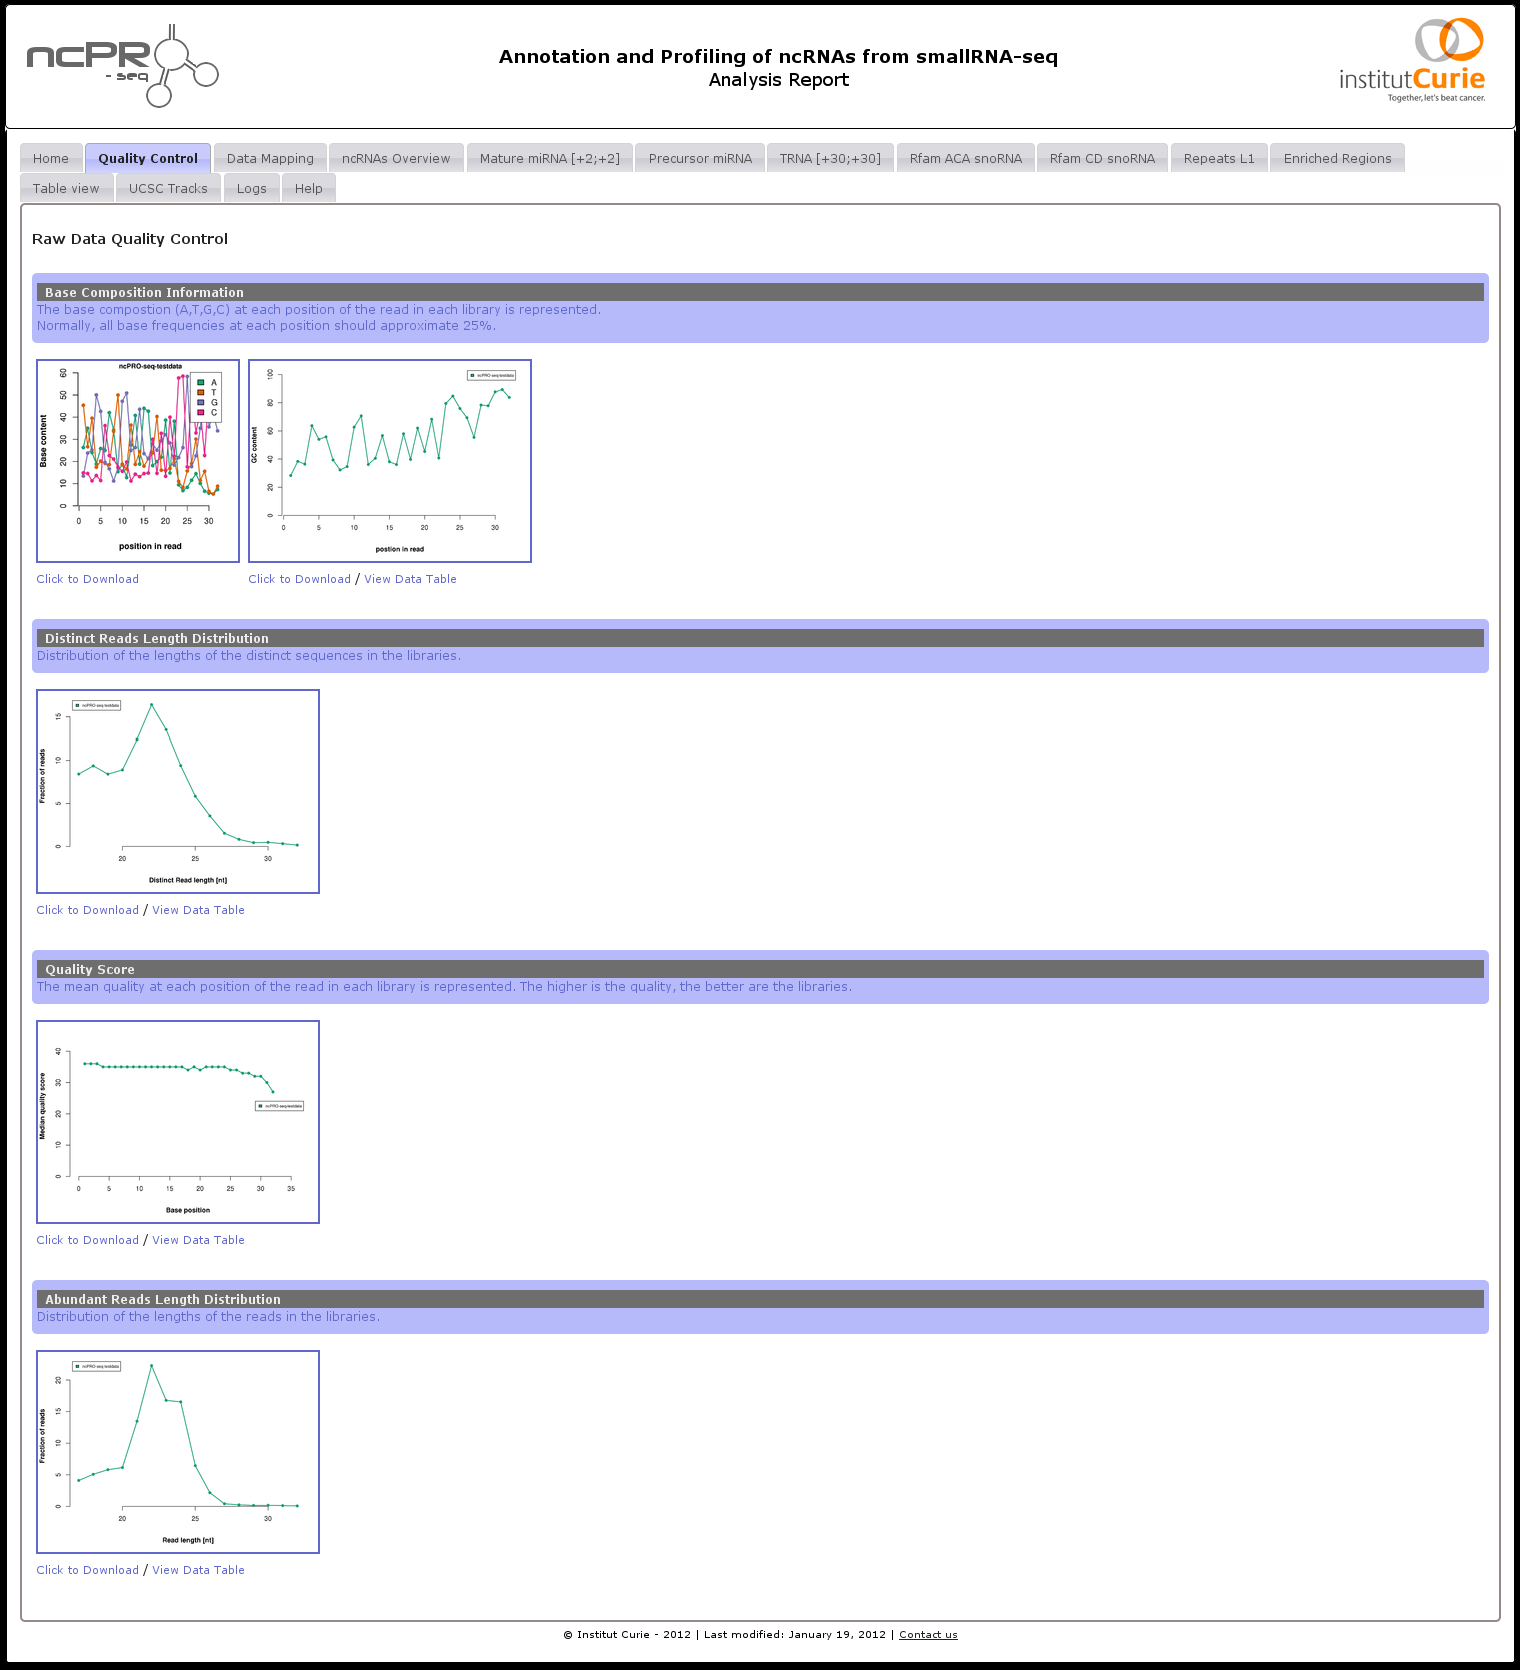
\includegraphics[width=\textwidth]{web_9.png}
\caption{\ncpip{} HTML analysis report}
\label{fig:report}
\end{figure}
\newpage

\section{How does-it work ?}

\subsection{Structure of the pipeline}
The workflow of the \ncpip{} pipeline consists of five main components: \textbf{input pre-processing}, \textbf{read mapping}, \textbf{read annotation}, \textbf{annotation analyses}, and \textbf{enrichment analyses}, as illustrated in Figure ~\ref{fig:pipelinestructure} with different background color. We will explain the tasks, key technical points and results of each step in the following subsections.
\begin{figure}[!h]
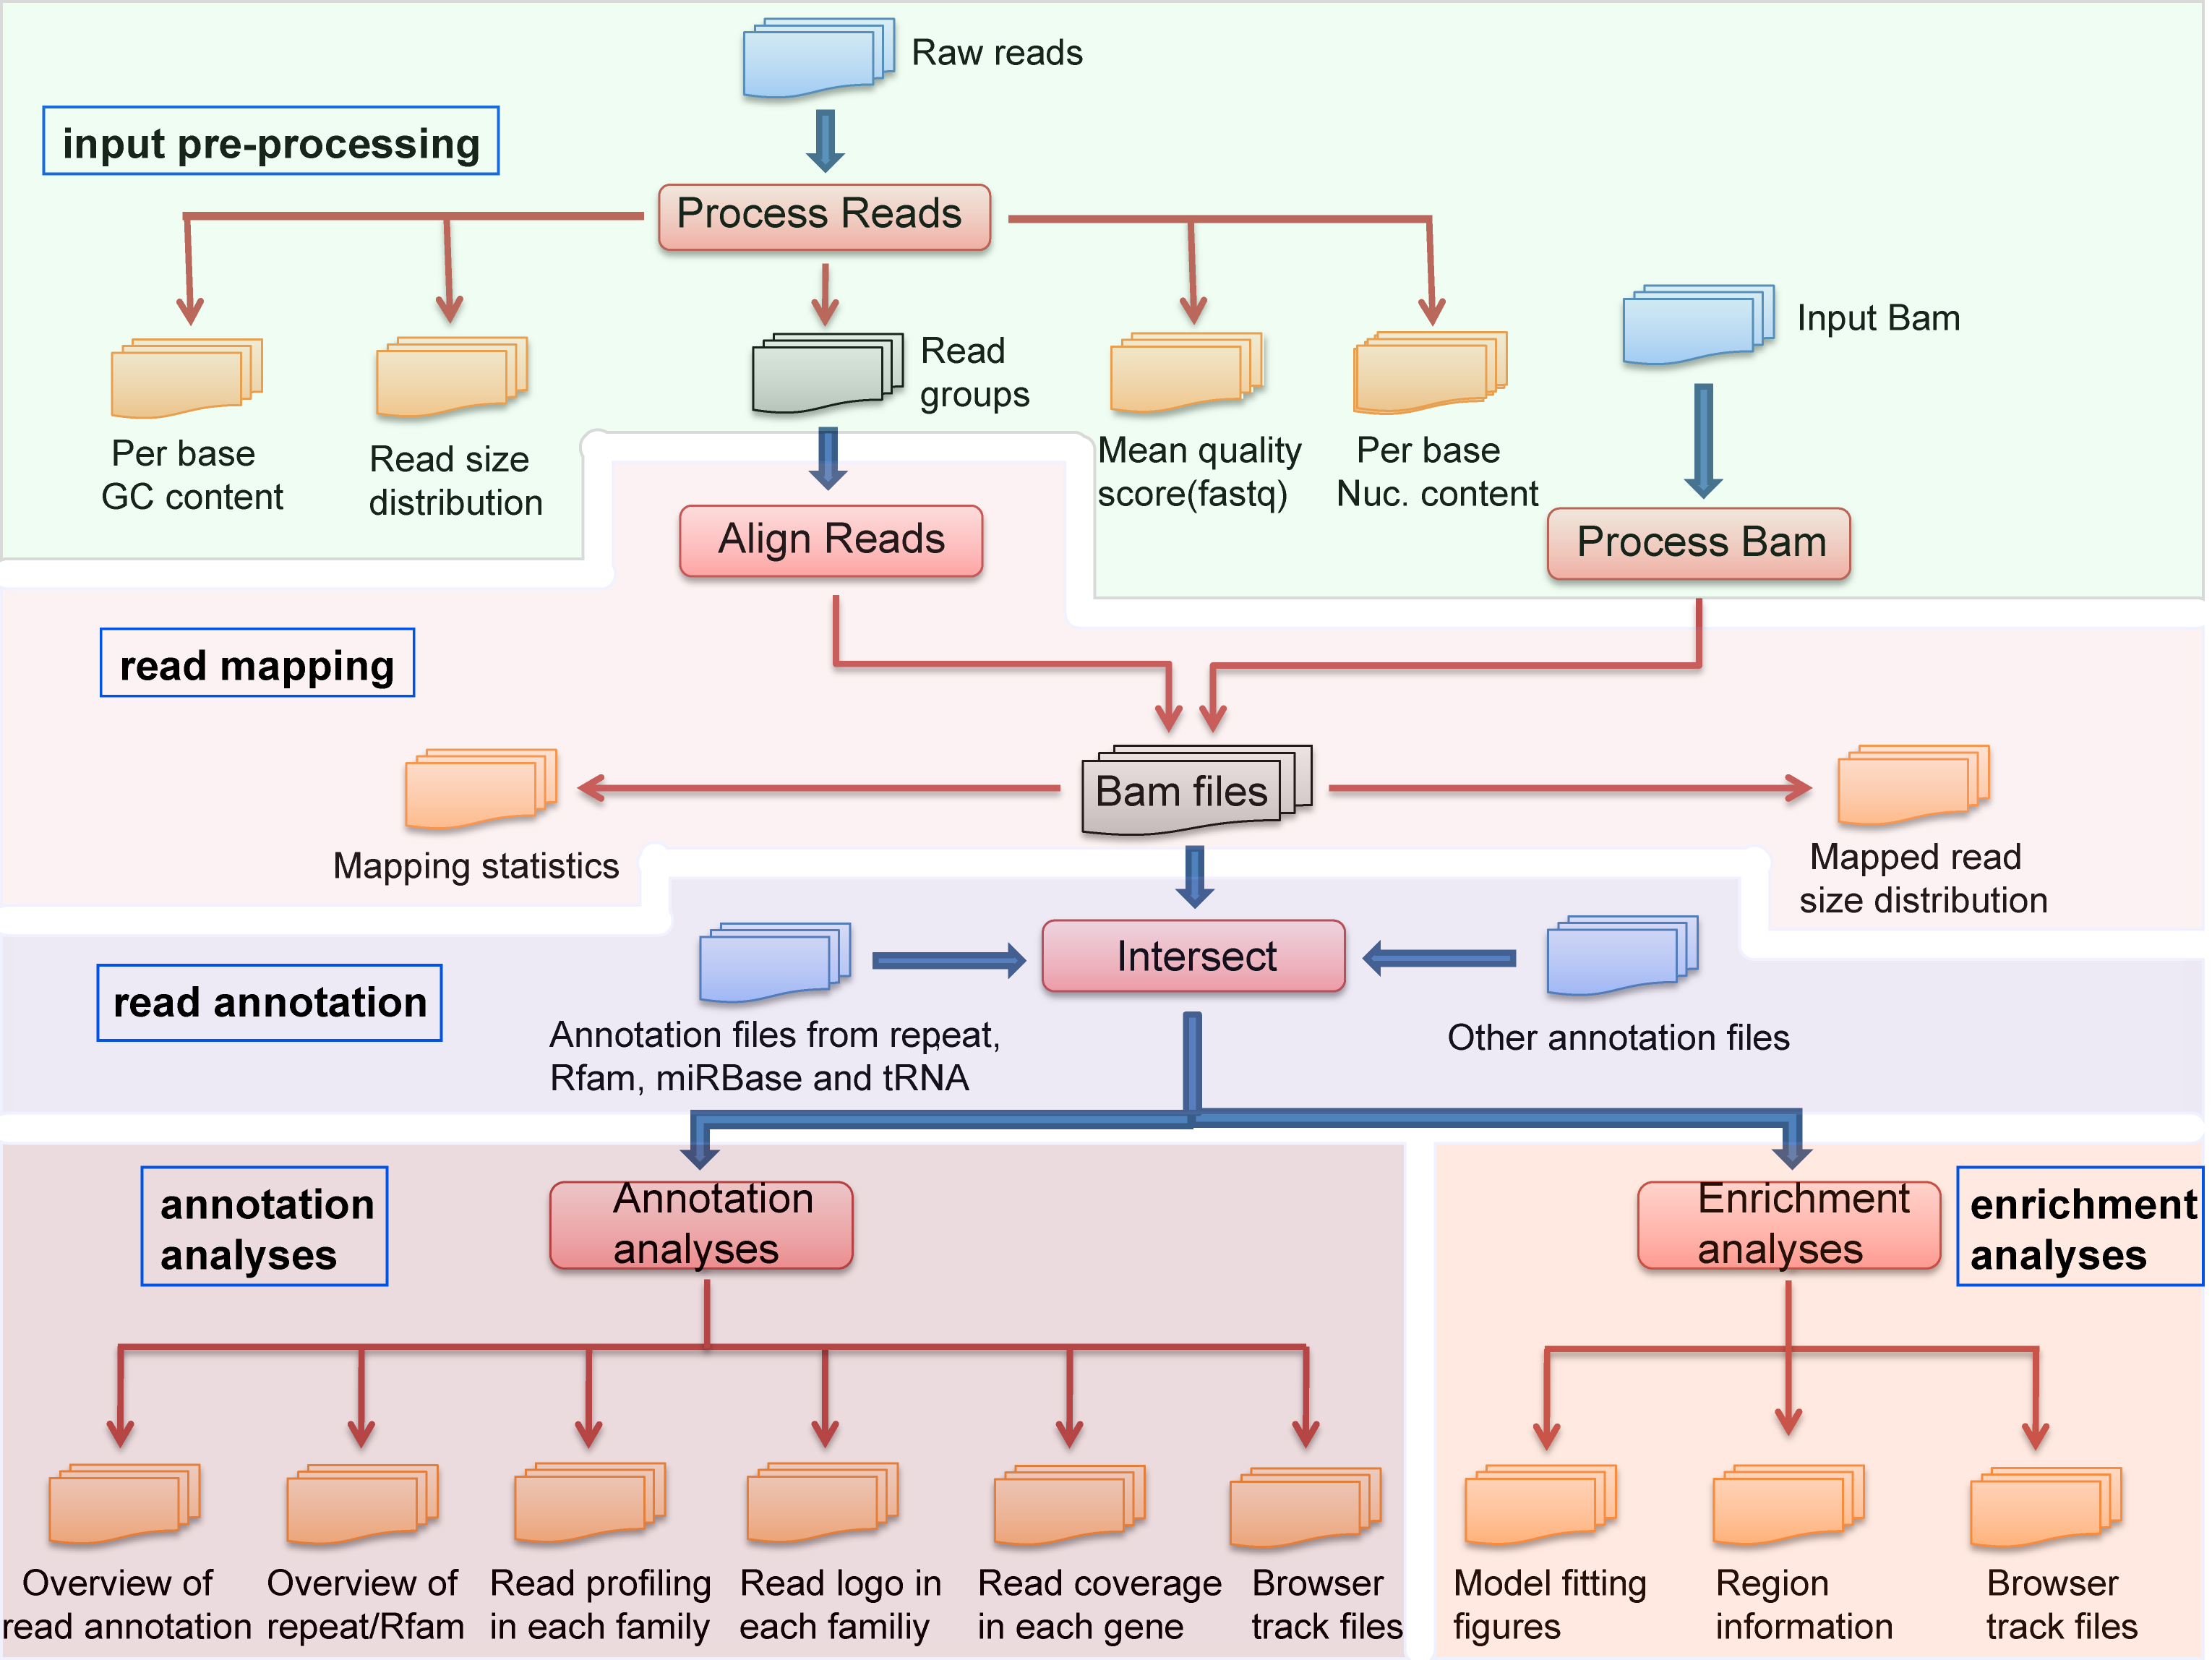
\includegraphics[width=160mm]{pipeline.png}
\caption{The whole workflow of \ncpip{}}
\label{fig:pipelinestructure}
\end{figure} 
\subsection{Input pre-processing}
Both read sequences and alignment results are acceptable as input in \ncpip{}. Input files are pre-processed before being sent to the next step.
\subsubsection{Read pre-processing}
\label{subsubsection:readpreprocess}
\ncpip{} supports input read sequences in three formats: \textbf{fastq} from Solexa, \textbf{csfasta} from SOLiD  and \textbf{fasta} from 454. In this step, \ncpip{} generates several figures for each sequencing library to describe the basic properties of sequencing reads, such as length distribution of distinct reads and abundant reads, positional base and GC content, and positional mean quality score if the read format is fastq, all of which are useful to access the basic quality of sequencing reads. Note that \textbf{distinct reads} are read groups that only count once for reads with the same sequence, i.e. ignoring the read abundance, whereas \textbf{abundant reads} are all sequenced reads. \\\\
There is an useful option in \ncpip{}, called \verb+GROUP_READ+ (see \ref{subsection:configure}), which controls the read clustering process. If it is set to 1, reads with identical sequence will be clustered into non-redundant read groups which are then specified with unique group id and read count. For reads in fastq format, the positional quality score of a read group is the mean positional quality score of all reads that are clustered in this group. In the following analyses, read groups, which has a significant decrease of read items comparing to the original read data, will be processed instead as input data. We recommend users to use this option especially if the sequencing libraries are extremely big, which will significantly reduce the CPU time for all analyses and the disk space as well to store intermediate results. Furthermore, another advantage of using this option is that you will get additional read profiles computed based on read groups (i.e. distinct reads) as shown in \ref{subsubsection:readprofile} 

\subsubsection{Alignment pre-processing}
\ncpip{} can also take read alignment files in BAM format as input. BAM is the compressed binary version of the SAM format, please check \href{http://samtools.sourceforge.net/}{ here} for more information. The \verb+GROUP_READ+ option also works for BAM file input. The clustering process is based on read sequences in alignments using the similar method as described in \ref{subsubsection:readpreprocess}. After this step, a new bam file will be generated by replacing original read information with read group and removing redundant alignments in original bam file.

\subsection{Reads mapping}
In \ncpip{}, \href{http://bowtie-bio.sourceforge.net/index.shtml}{ Bowtie} ($<$v2) \cite{Langmead2009} is used to align reads to the reference genome. Different bowtie options can be specified to map different formats of reads: \verb+BOWTIE_GENOME_OPTONS_FQ+ for fastq reads, \verb+BOWTIE_GENOME_OPTIONS_FA+ for fasta reads and \verb+BOWTIE_GENOME_OPTIONS_CS+ for csfasta reads. Bowtie outputs alignments in SAM format, which are then converted to BAM format by using \href{http://samtools.sourceforge.net/}{ SAMtools} \cite{Li2009}. \\\\
Both BAM files from read alignment and from input BAM file pre-processing step will be used to generate figure files summarizing mapping information: mapping statistics and mapped read size distribution. In the mapping statistics figure, the proportions of reads with unique and multiple mapping sites in the genome, and unmapped reads are plotted. 

\subsection{Reads annotation}
To find overlaps between read alignments and genomic annotations, intersectBed tool in \href{http://code.google.com/p/bedtools/}{ BEDTools} \cite{Quinlan2010} is implemented. Only read alignments which have 100\% overlap with annotations are reported by setting -f option in intersectBed to 1. \\For reads which can be annotated as given genomic features, detail analyses as shown below will be performed. We also explain the way how we deal with reads with multiple mapping sites and how coordinates of genomic features can be modified.

\subsubsection{Reads with multiple mapping sites}
A major challenging problem using NGS sequencing data is the annotation of reads aligned at multiple locations. Most of the available frameworks resolve this situation by discarding these reads or by providing random annotations. Here, we propose to keep all the reads aligned to the genome, and to weight them by the number of mapping sites. Suppose a read can be aligned 5 times to the genome, for each mapping site, the read would be counted as 0.2, i.e. 1/5.

\subsubsection{Extension parameters}
\label{subsubsection:extension}
There are four types of extended items which can be used to modify coordinates according to the pattern \verb|\_[iest]\_[+-]Number\_[+-]Number|, as illustrated in Figure ~\ref{fig:coordinatemod}: 
\begin{enumerate}
\item \textbf{\_i\_[+-]N1\_[+-]N2}: shorten [+-]N1 bp at 5' end, [+-]N2 bp at 3' end
\item \textbf{\_e\_[+-]N1\_[+-]N2}: extend [+-]N1 bp at 5' end, [+-]N2 bp at 3' end 
\item \textbf{\_s\_[+-]N1\_[+-]N2}: get coordinates for sub-region from position N1 to N2 indexed from 5' end 
\item \textbf{\_t\_[+-]N1\_[+-]N2}: get coordinates for sub-region from position N1 to N2 indexed from 3' end
\end{enumerate}
\begin{figure}[!h]
\setlength{\unitlength}{5cm}
\begin{picture}(3,1)(0,0.1)
\color{red}
\linethickness{3mm}
\put(0.5,0.6){\line(1,0){2}}
\color{green}
\linethickness{1mm}
\put(0.2,0.4){\line(1,0){0.5}}
\color{green}
\linethickness{1mm}
\put(2.2,0.4){\line(1,0){0.5}}
\color{green}
\linethickness{1mm}
\put(0.7,0.2){\line(1,0){1.5}}
\color{green}
\linethickness{1mm}
\put(0.2,0.8){\line(1,0){2.5}}
\color{gray}
\linethickness{0.5mm}
\multiput(0.2,0.1)(0,0.1){9}{\line(0,1){0.05}}
\color{gray}
\linethickness{0.5mm}
\multiput(0.5,0.1)(0,0.1){9}{\line(0,1){0.05}}
\color{gray}
\linethickness{0.5mm}
\multiput(0.7,0.1)(0,0.1){9}{\line(0,1){0.05}}
\color{gray}
\linethickness{0.5mm}
\multiput(2.2,0.1)(0,0.1){9}{\line(0,1){0.05}}
\color{gray}
\linethickness{0.5mm}
\multiput(2.5,0.1)(0,0.1){9}{\line(0,1){0.05}}
\color{gray}
\linethickness{0.5mm}
\multiput(2.7,0.1)(0,0.1){9}{\line(0,1){0.05}}
\put(0.41,0.93){\vector(1,0){0.09}}
\put(0.29,0.90){$N1$}
\put(0.29,0.93){\vector(-1,0){0.09}}
\put(0.66,0.93){\vector(1,0){0.04}}
\put(0.54,0.90){$N2$}
\put(0.54,0.93){\vector(-1,0){0.04}}
\put(2.41,0.93){\vector(1,0){0.09}}
\put(2.28,0.9){$N3$}
\put(2.29,0.93){\vector(-1,0){0.09}}
\put(2.67,0.93){\vector(1,0){0.04}}
\put(2.54,0.9){$N4$}
\put(2.54,0.93){\vector(-1,0){0.04}}
\put(0.43,0.57){$0$}
\put(2.54,0.57){$L$}
\put(0.74,0.38){$\emph{\_s\_-N1\_+N2}$}
\put(2.74,0.38){$\emph{\_t\_-N3\_+N4}$}
\put(1.3,0.08){$\emph{\_i\_+N2\_+N3}$}
\put(2.74,0.78){$\emph{\_e\_+N1\_+N4}$}
\end{picture}
\caption{The four types of modification based on the original coordinates}
\label{fig:coordinatemod}
\end{figure}

Note that for repeat annotation, extension operations will only perform on the full length repeat in the genome. That means repeat items in the \verb+NCRNA_RMSK_EX+ option (see \ref{subsection:configure}) if it is specified will only select untruncated repeats to do the modification and analyses. Repeats representing $>=90\%$ of its consensus sequence are considered as full length/untruncated repeats.\\\\
Here, we show two examples of extension parameters use:
\begin{description}
 \item[Annotate reads in mature miRNAs.] Due to the inaccurate processing of precursor miRNAs by Dicer or downstream miRNA remodelling, mature miRNAs often have end heterogeneities comparing to their annotations in miRBase. Thus, when analyzing mature miRNAs, it is necessary to extend miRNA annotation several bases (e.g. 2 bases) in both upstream and downstream region, which can be easily done in \ncpip{} by using \textbf{miRNA\_e\_+2\_+2}.
 \item[Analyse tRNA-derived small RNAs (tsRNAs).] It has been reported that tRNA can be processed again into different types of small RNAs probably through different mechanisms. To check read profiles of these small RNA families, you can specify the following options to \textbf{TRNA\_UCSC} separated by comma: \textbf{tRNA\_e\_+0\_+50} (overview of all tsRNAs), \textbf{tRNA\_s\_+0\_+26} (tsRNAs at very 5' end), \textbf{tRNA\_s\_+0\_+40} (including tsRNAs from tRNA anti-codon stem cleavage) and \textbf{tRNA\_t\_+0\_+50} (tsRNAs from 3' tail of precursor tRNAs).
 \end{description}

\subsubsection{miRNAs read proportion}
\label{subsubsection:mirnaread}
In this step, abundant reads mapped in mature miRNA regions are counted, and plotted as the proportion of all mapped reads in the genome. The annotation file of mature miRNA is generated using files from miRBase \cite{Kozomara2011} detailed in \ref{subsection:mirna}. Each miRNA count is calculated using the intersection of the reads alignement with the mature positions (see intersectBed program from BEDTools).

\subsubsection{Reads annotation overview}
The reads annotation family is the most general overview, and counts the reads based on the following annotations : coding genes, ncRNAs from Rfam, smallRNAs from repeated regions, rRNAs, and precursor miRNAs from miRBase. One read can belong to several annotations (see multiIntersectBed from BEDTools).

\subsubsection{Overview of repeat/Rfam}
\label{subsubsection:overview}
To compare the read expression in different repeat/Rfam families, we count the number of abundant reads in each family and plot the relative proportion.
\begin{description}
 \item[Rfam] We catalogue non-coding RNA genes in Rfam annotation into five big classes: tRNA, rRNA, snRNA, ACA\_snoRNA, CD\_snoRNA and others. Note that miRNA annotations are excluded in the Rfam noncoding RNA analyses, for the reason that we have already obtained the miRNA read mapping information in \ref{subsubsection:mirnaread}. All rfam annotation files are downloaded from Rfam database \cite{Gardner2011}, please see section \ref{subsection:rfam} for more details.
 \item[Repeat] \ncpip{} uses repeat annotations from \href{http://www.repeatmasker.org/}{ RepeatMasker} \cite{Smit2008} results, see section \ref{subsection:repeat} for the preparation of the annotation file. We classify different repeats based on the name of repeat family.
 \end{description}


\subsubsection{Read profiling in each family}
\label{subsubsection:readprofile}
Read profiling refers to the analysis of read profiles, which are represented by the distribution of positional read coverage and the read length distribution in annotation family. If the \verb+GROUP_READ+ option is activated,  for each annotation family, we will compute and plot two types of read profiles, by using abundant and distinct reads respectively, or else only read profiles based on abundant reads will be investigated. \\\\
In read profiles, three types of read coverage distribution, which are generated based on 5' end, 3' end and all positions of reads respectively, are displayed together to have a clear view of the biogenesis of small RNAs. Since annotated features belonging to the same single family might have different full length, we use a scaling strategy as shown in Figure \ref{fig:scaling} to transform read positions in annotated items to corresponding positions in the scaled region. Using this strategy, we are able to sum up positional read coverages from different annotated features in a family, which are then normalized by the number of occurences of each feature position in the genome to obtain the average positional read coverage distribution. For repeat families, additional process is applied before the scaling step that is to locate the annotated repeat regions to the consensus sequence of its family, since repeats from some family like L1 in mouse are always truncated in the genome.  Note that the occurrence of read is normalized by the total number of either mapped abundant reads or mapped distinct reads to RPM (reads per million mapped reads) depending on the type of read profiles. We then plot the average read coverage distribution in the scaled region, and number the X-axis according to the median size of annotated items in the family.\\\\
In each type of read profiles, relative length distributions of reads mapped in the sense, antisense and both direction of annotation family are plotted.

\begin{figure}[h!]
\begin{center}
 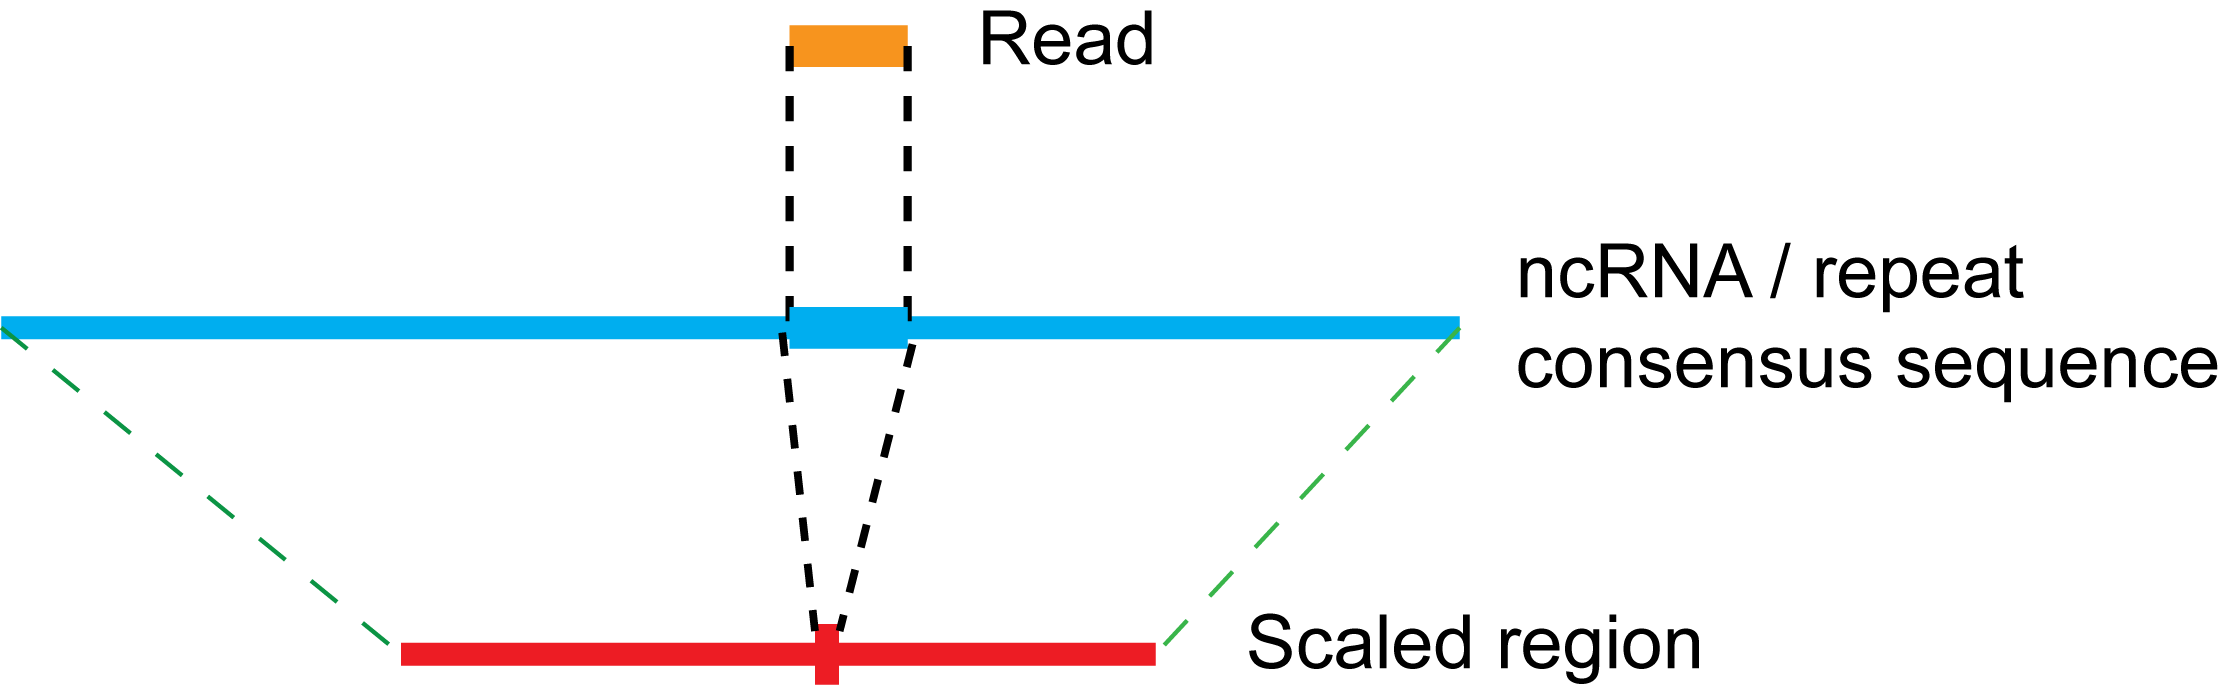
\includegraphics[width=160mm]{scaling.png}
 % scaling.png: 2219x693 pixel, 300dpi, 18.79x5.87 cm, bb=0 0 533 166
\end{center}
\caption{The scaling process}
\label{fig:scaling}
\end{figure} 
\subsubsection{Logo sequences}
\label{subsubsection:logo}
It is interesting to investigate the base bias in distinct reads from each annotation family, which might give hints about how these small RNAs are processed. In \ncpip{}, we calculate the frequencies of bases at each position of distinct reads and plot them in \href{http://www.bioconductor.org/packages/2.2/bioc/html/seqLogo.html}{ sequence logos} \cite{OliverseqLogo}. Sequence logos can be drawn with respect to 5' end or 3' end of reads depending on the choice of \textbf{5} or \textbf{3} in \verb+LOGO_DIRECTION+ option. Users can choose their favourite way to display sequence logos, either with uniform column heights, or with column heights proportional to informaion content. (\verb+IC_SCALE+ option). \\\\
For each annotation family, \ncpip{} provides two types of sequence logos figures by using different subsets of distinct reads. In one figure, all distinct reads in annotation family are used to create sequence logos, which will give you the processing information of small RNAs like piRNAs that can be produced from various positions in a single region. In another figure, only the distinct read with the highest abundance in each family member is used, which is the case for small RNAs like miRNAs that are accurately processed by enzymes from some special loci. 

\subsubsection{Read coverage in each annotation item}
For each annotation family including different repeat/Rfam families and other custom annotations, \ncpip{} creates a table file showing read coverages of each single family member in all sequencing libraries. These table files are compatible with R package like DESeq \cite{Simon2010} to identify significantly expressed family members. For instance, you can find read coverage of each miRNA gene in the miRNA table file. Note that in the tRNA table file, read coverages are computed based on types of tRNA instead of single tRNA genes, since several studies found that expressions of tRNA-derived small RNAs differ from one type of tRNA to another.

\subsubsection{Track files}
For each sequencing library,  for each annotation family, \ncpip{} generates compressed track files in both \href{http://genome.ucsc.edu/goldenPath/help/bedgraph.html}{bedgraph} and \href{http://genome.ucsc.edu/goldenPath/help/bed.html}{bed} formats to describe read mapping in sense and antisense direction of annotation items respectively. \\\\
As we have listed in \ref{subsection:configure}, there is an option called \verb+GENOME_TRACK_OPTIONS+ which allow users to select different subsets of reads mapped in the genome to generate BedGraph formatted track files.\\\\
In BedGraph formatted track files, read coverage is computed for each genomic position. \\\\
All track files outputed from \ncpip{} can be directly uploaded to \href{http://genome.ucsc.edu/index.html}{ UCSC browser} / other genome browser for visualization.

\subsection{Enrichment analysis}
\label{subsection:enrichmentanalysis}
\ncpip{} has a special engine, which we call \textbf{enrichment analysis}, to analyse reads that can not be annotated as known genomic features. Users can select different subsets of reads to perform this analysis by giving different sets of options to \verb+SIG_READ_OPTIONS+ (section \ref{tab:configureoptions}). And reads that can be aligned to annotation regions given in \verb+EXCLUDE_ANN_GFF+ are excluded from enrichment analysis. Finally, we use the following steps to identify regions significantly enriched with remaining reads after filter steps.

\begin{enumerate}
 \item Slide window of fixed size  (\verb+SIG_WIN_SIZE+, e.g. 100,000) along the whole genome at fixed step (\verb+SIG_STEP_SIZE+, e.g. 50,000)
 \item For each window, summarize read mapping information (number of mapped reads\ldots)
 \item Fit number of mapped reads in all window to selected model to estimate expected read number distribution
 \item Compare real and expected read number distribution to determine P value for each window, thereby identify regions with significant numbers of mapped reads (\verb+PVAL_CUTOFF+, e.g. 0.001)
 \item Finally generate tables containing read information and additional gene annotation of these regions. Track files in \href{http://genome.ucsc.edu/FAQ/FAQformat.html#format1}{bed} format are also created
\end{enumerate}

There are three models that users can choose to do simulation and fit sliding window results: 
\begin{enumerate}
 \item NB.ML: negative binomial distribution inferred using maximum likelihood method
 \item NB.012: negative binomial distribution inferred using windows with only 0, 1, or 2 aligned reads
 \item Poisson: Poisson distribution inferred using windows with only 0, 1, or 2 aligned reads
\end{enumerate}

For more details about these three models, please check the \verb+addNBSignificance+ function in \href{http://www.bioconductor.org/packages/2.6/bioc/html/girafe.html}{ girafe} R package \cite{Joern2010}.\\

In this step, three types of results are generated: figures displaying the distribution of sliding windows with different number of reads mapped and model simulation results, table files containing location, read mapping and annotation information of identified regions significantly enriched with reads, and track files in \href{http://genome.ucsc.edu/FAQ/FAQformat.html#format1}{bed} format.

Note that for small genomes and plant genomes, please choose small sliding window, as big window might lead to the problem of non-existance of window with less than 2 or 10 reads which is important for the model simulation.

\section{Annotation files}

In \ncpip{}, we have already genearated noncoding RNA/repeat annotation files for some ($>=15$) model organisms, including Human,Mouse,Rat, Arabidopsis, Caenorhabditis elegans, Drosophila melanogaster, etc. Please refer to \href{http://ncproseq.sourceforge.net/download.html}{ our project website} for a complete list of available species. \\If users want to create annotation files by themselves in case of working on other speicies or for special usages, please follow the instructions below and refer to readme in annotation/prepareAnnotation folder for commands used to generated these files. Note that \ncpip{} only accepts annotation files in \href{http://gmod.org/wiki/GFF#GFF3}{ gff3} format. 

\subsection{Rfam annotation}
\label{subsection:rfam}
Rfam annotation file can be directly downloaded from \href{ftp://ftp.sanger.ac.uk/pub/databases/Rfam}{ Rfam database} \cite{Gardner2011}. Since the reference genomes of some species might changes in different version of Rfam database, make sure that you are using the right Rfam annotation file for your genome assembly. For example, the latest Rfam annotation file for NCBI37/mm9 mouse genome is in version 9.0, but not version 10 where you can find the annotation file for GRCh37/hg19 human genome. If there is a conflict between the genome assembly used by Rfam and the one you are analyzing, we offer a simple and quick way to solve it by generating new Rfam annotation file for your genome assembly. Basically, we extract Rfam sequences based on the genome annotation in Rfam, then blast them to the new genome, finally use rfam\_scan.pl from Rfam database and custom script to create new Rfam annotation file from blast results. And another way to avoid the conflict is: if you have the chain file specifying differences between two different genome assemblies, you can use liftOver from UCSC genome website to get new rfam gff file. \\\\
In Rfam annotation file, the value in "Alias" tag in the "attributes" column indicates the ncRNA family information. Example of "attributes" column:\\\\
\verb|ID=RF00026.1;Name=RF00026;Alias=U6;Note=AC157543.8/131368-131259|

\subsection{RepeatMasker annotation}
\label{subsection:repeat}
The repeat annotation file is generated from the ouput of RepeatMasker \cite{Smit2008}. Users can use our custom scripts to create repeat gff3 file either from UCSC genome browser or from local RepeatMasker output, which are detailed in readme file in annotation/prepareAnnotation folder\\\\ 
There are a list of special feature attributions in repeat annotation files. The "repName","repClass" and "repFamily" features indicate the name, class and family of the repeat respectively. The other three features are used to indicate the location of repeat region in consensus sequence. \\\\
Example of "attributes" column:\\\\
\verb|repName=L1_Mur2;repClass=LINE;repFamily=L1;repSt=1413;repEnd=1567;| \\
\verb|repFullLen=5877;|

\subsection{miRNA annotation}
\label{subsection:mirna}
The miRNA annotation files used in \ncpip{} are created based on files from miRBase \cite{Kozomara2011}. The precursor miRNA gff file downloaded from miRBase can be used in \ncpip{} after being transformed from gff2 to gff3 format. In miRBase, we cannot find genome coordinates of mature miRNAs. Therefore, we wrote a custom script to generate mature miRNA annotation file based on the mature miRNA sequences, precursor miRNA sequences and precursor miRNA annotation file. \\\\
Example of "attributes" column in precursor miRNA annotation file:\\\\
\verb|ACC=MI0006363;ID=hsa-mir-1302-2|\\\\
Example of "attributes" column in mature miRNA annotation file:\\\\
\verb|Name=mmu-miR-206*;Precursor=mmu-mir-206;ID=mmu.miR.206star|

\subsection{tRNA annotation}
\label{subsection:trna}
The tRNA annotation file is generated from tRNA gtf files from UCSC \cite{Dreszer2012} using custom scripts, detailed in readme file in annotation/prepareAnnotation folder. There is a feature in "attributes" column called "Type\_Name" which indicate the type of tRNA. Example of "attributes" column: \\\\
\verb|ID=chr1.tRNA1547;Type_Name=tRNA-GluTTC|

\subsection{Other annotations}

While "nc" in the name implies a focus on noncoding RNAs, \ncpip{} is far more and can be used to analyse any annotation files in gff3 format like splice site and promoter region of protein coding gene. Note that these annotation files should contain one of the following three features in "attributes" column to indicate the names of items: Name, Alias or ID. \\\\
It has already been reported that small RNAs are enriched at 3' ends of internal exons (spliRNAs) and at transcription initiation sites (tiRNAs) \cite{Taft2010}. To show how the "other annotations" option works, we create gff3 annotation files of both splice donor site and acceptor site for genomes that has refgene annotation in UCSC \cite{Dreszer2012}. Basically, to generate donor site annotation, we locate the 3' end of all exons except the last one in genes, and extend 100bp upstream and downstream, thereby obtain regions of size 201bp with 3' end of exon at position 101. For acceptor site, 5' end of exons excluding the first exon in genes are chosen to extend +- 100bp. \\\\
Example of "attributes" column in splice acceptor annotation file:\\\\
\verb|GeneName=NM_001083312;Exon_idx=2;Type=acceptor;Extend_base=100;|\\\\
Example of "attributes" column in splice donor annotation file:\\\\
\verb|GeneName=NM_001083312;Exon_idx=1;Type=donor;Extend_base=100;|

\section{Installation of additional softwares}
\label{subsection:additional}

We give some simple outlines to install additional  softwares required by \ncpip{}, for more information, please refer to the main site of each software:

\begin{itemize}
 \item The \href{http://bowtie-bio.sourceforge.net/manual.shtml}{ Bowtie Aligner} ($<$v2.0) \cite{Langmead2009}.

\begin{itemize}
 \item The latest Bowtie program can be found \href{http://sourceforge.net/projects/bowtie-bio/files/bowtie/0.12.7}{ here}. Users can choose the pre-compiled version for your operating system, or build your own Bowtie from the source (bowtie-*-src.zip). Users need to unzip the downloaded file. If starting with the source, users should use \verb+make+ command at the shell prompt to compile the program. In both ways, users should either add the directory where Bowtie binaries are located to your \verb+PATH+ variable, or copy/move Bowtie binaries to a directory (e.g. /usr/local/bin) in your \verb+PATH+ variable.\\\\
The indexes of the chosen genome reference need to be prepared beforehand and set in the environment variable \verb|BOWTIE_INDEXES|
\end{itemize}

 \item The \href{http://www.r-project.org/}{ R} ($>$v2.12.0) \cite{Rcitation} and \href{http://www.bioconductor.org/}{ BioConductor} \cite{Robert2004} softwares.

\begin{itemize}
 \item There are several ways to install R program detailed in \href{http://cran.r-project.org/doc/manuals/R-admin.html#}{ R-project site}. For Mac OS X, the easiest way is to download the latest installer package (R-*.pkg) for Mac OS X, which can be installed by double clicking.  For Linux, we just show how to build R from the source.  Users can choose a \href{http://cran.r-project.org/mirrors.html}{ site mirror} close to you to download the latest R source code (R-*.tar.gz) for all platforms. You need to unpack the file and go to the unpacked directory at the shell prompt, use
\begin{verbatim}
> ./configure
> make
> su
> make install
\end{verbatim} 
\end{itemize}

\begin{itemize}
 \item To install Bioconductor, make sure that your computer is connecting to internet and use the following commands in an R command window (type \verb+R+ in your shell prompt, and press enter$ \hookleftarrow $):
\begin{verbatim}
> source("http://bioconductor.org/biocLite.R")
> biocLite()
\end{verbatim} 
\end{itemize}

 \item The R packages:  \href{http://www.bioconductor.org/packages/2.2/bioc/html/seqLogo.html}{ seqLogo} \cite{OliverseqLogo}, \href{http://www.bioconductor.org/packages/2.6/bioc/html/girafe.html}{ girafe} \cite{Joern2010} and  \href{http://cran.r-project.org/web/packages/RColorBrewer/index.html}{ RColorBrewer} \cite{Erich2011}.

\begin{itemize}
 \item To install the seqLogo and girafe package in R, use the following commands in an R command window:
\begin{verbatim}
> source("http://bioconductor.org/biocLite.R")
> biocLite("girafe")
> biocLite("seqLogo")

\end{verbatim} 
 \item To install the RColorBrewer package in R, use the following command in an R command window:
\begin{verbatim}
> install.packages("RColorBrewer")
\end{verbatim} 
\end{itemize}

 \item The \href{http://code.google.com/p/bedtools/}{BEDTools suite} ($>=$v2.15.0) \cite{Quinlan2010} and the \href{
http://xfer.curie.fr/get/nil/2Rpz9IfJKcZ/BEDTools_MapCount_ColorTag.tar.gz}{ bamMapCount} program.

\begin{itemize}
 \item The latest BEDTools can be downloaded \href{http://code.google.com/p/bedtools/downloads/list}{ here} (BEDTools.*.tar.gz). Use the following commands to compile BEDTools, and copy/move all binaries in bin subdirectory to a directory (e.g. /usr/local/bin) in your \verb+PATH+ variable
\begin{verbatim}
> tar -zxvf BEDTools.<version>.tar.gz 
> cd BEDTools<version>
> make clean
> make all
> su
> cp bin/* /usr/local/bin
\end{verbatim} 
\end{itemize}

\begin{itemize}
 \item The bamMapCount program is friendly shared by Assaf Gordon, which can be found \href{http://xfer.curie.fr/get/2Rpz9IfJKcZ/BEDTools\_MapCount\_ColorTag.tar.gz}{ here} (BEDTools\_MapCount\_ColorTag.tar.gz). He integrated his programs to BEDTools. Users can unpack the whole package and compile it, then just copy/move the bamMapCount program in bin subdirectory to a directory (e.g. /usr/local/bin) in your \verb+PATH+ variable if you have already installed BEDTools.
\begin{verbatim}
> tar -zxvf BEDTools_MapCount_ColorTag.tar.gz
> cd BEDTools_MapCount_ColorTag
> make all
> su
> cp bin/bamMapCount /usr/local/bin
\end{verbatim}
\end{itemize}

 \item The \href{http://samtools.sourceforge.net/}{ SAMTools suite} \cite{Li2009}.

\begin{itemize}
 \item Users can download the latest version of SAMtools \href{http://sourceforge.net/projects/samtools/files/latest/download?source=files}{ here} (samtools-*.tar.bz2). Make sure that you have \href{http://www.zlib.net}{ zlib} library ($>$v1.2.3) installed in your system before compiling SAMtools. Then use the following commands to compile the SAMtools packages, and copy/move 'samtools', `bcftools/bcftools' and other executables/scripts in `misc' to a directory (e.g. /usr/local/bin) in your \verb+PATH+ variable: 
\begin{verbatim}
> tar -xvjpf samtools-<version>.tar.bz2
> cd samtools-<version>
> make
> su
> cp samtools /usr/local/bin
> cp bcftools/bcftools /usr/local/bin
\end{verbatim} 
\end{itemize}

 \item The \href{http://www.imagemagick.org/script/index.php}{ Convert/ImageMagick} utilies.

\begin{itemize}
 \item The Convert/ImageMagick normally comes with most of modern linux/UNIX systems, but if you also want to install another version, there are a few easy steps to do which are detailed \href{http://www.imagemagick.org/script/install-source.php#unix}{ here}. For Mac OS X, users can use \href{http://www.macports.org/}{ MacPorts} command as shown below to build ImageMagick in your system.
\begin{verbatim}
> su
> port install ImageMagick 
\end{verbatim}
\end{itemize}

 \item A local server with php.

\begin{itemize}
 \item We recommend users to install \href{http://www.apachefriends.org/en/xampp.html}{ XAMPP}, a free and open packages consisting Apache, MySQL, and Perl/PHP/Python. To install XAMPP, you just need to download the right software version for your system and extract it. For linux/UNIX, download XAMPP and follow steps in this \href{http://www.apachefriends.org/en/xampp-linux.html}{ page}. For Mac OS X, check this \href{http://www.apachefriends.org/en/xampp-macosx.html}{ page}
\end{itemize}

\end{itemize}

\section{FAQ}
\subsection{Enabling CGI using XAMPP}
If not well configured, the server can send a "Error 403 Access forbiden" during the CGI execution.\\
This could happen for instance with the file browser system of \ncpip{}. To correct the error, be sure that the httpd.conf file of XAMPP is well configured.
For instance, on MacOS, edit the file /Application/XAMPP/etc/httpd.conf and add the following parameters.
\begin{verbatim}
<Directory "/Applications/XAMPP/xamppfiles/cgi-bin/">
    AllowOverride None
    Options Indexes FollowSymLinks MultiViews ExecCGI
    Order allow,deny
    Allow from all
</Directory>
\end{verbatim}
This will enabling the CGI to be executed.

\subsection{Working with a new genome}

In \ncpip{}, it is possible to do small RNA profiling analyses in a new genome without giving any known annotations (miRNA, tRNA, etc). For example, you want to work in yeast. What you need to do is:
\begin{enumerate}
 \item create the bowtie index of yeast genome with index name "yeast", put them in your Bowtie index folder
 \item create a folder "yeast" in MY\_INSTALLATION\_DIR/annotation directory
 \item create the "chrom.sizes" file of your yeast genome in MY\_INSTALLATION\_DIR/annotation/yeast folder. "chrom.sizes" is the reference idex file, which has two columns (name of chromosome and size of the chromosome) and can be generated using samtools 
\end{enumerate}


\newpage
%\section{References}
%\renewcommand*{\refname}{}
\addcontentsline{toc}{section}{Bibliography}

\bibliographystyle{plain}
\bibliography{manual}
\nocite{*}


\end{document}